\documentclass[a4paper,11pt]{article}
\usepackage{graphicx}
\usepackage[utf8]{inputenc}
\usepackage{hyperref}
\usepackage{placeins}
\usepackage[newfloat]{minted}
\usepackage{caption}

\newenvironment{code}{\captionsetup{type=listing}}{}
\SetupFloatingEnvironment{listing}{name=Code Overview}


\hypersetup{
    colorlinks=true,
    linkcolor=blue,
    filecolor=black,      
    urlcolor=blue,
    citecolor=black,
}
\begin{document}

\title{
    \textbf{Linked List Report.}
}
\author{Adrian Jonsson Sjödin}
\date{Fall 2022}

\maketitle

\section*{Introduction}
The purpose of this assignment is to gain a better understanding of pointers and references
and how they can be used to create more complicated data structures. In particular we will
gain a deeper understanding of how linked lists functions.

\section*{Task}
Implement a linked list class from the ground up that utilizes a stack structure. Also
create a method that allows one to append another linked list to said created linked list.
Having implemented that, benchmark the run time of the append operation. Vary the size of the
first linked list \textbf{a} and append it to a fixed size linked list \textbf{b} and
examine how the run time changes with the size of list \textbf{a}.

Lastly implement the equivalent append operation using arrays and benchmark this operation.
How does this compare to the append operation for the linked list class? Without doing any measurements, 
describe the difference in execution time for this linked list stacked as compared to the stack implemented 
using arrays from the previous assignment.

\section*{Method \& Theory}
I implemented the linked list stack using a private helper class to create nodes that contains the value 
we want to add to the list, and a pointer to the next node in the list. So when a linked list are created 
it is created empty and when we want to add a value to it we create a new node that will then have a pointer
\textit{next} that will be null for the first node. But since every new node will be created and added to the 
left of it in the list, they will have a pointer to the previous node already in the list. Figure 
\ref{fig:linkedListDiagram} shows how this would look like and code overview \ref{code:classStructure} shows the code implementation
of this.

\begin{figure}[h]
    \centering
    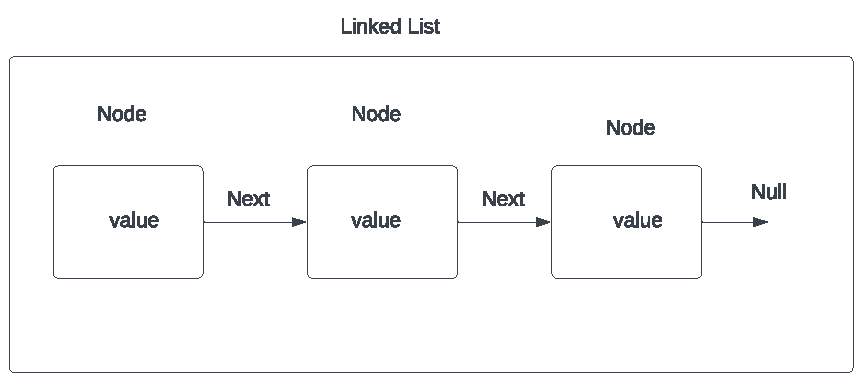
\includegraphics[width=\textwidth]{linkedListDiagram.pdf}
    \caption{Depiction of node implementation in a linked list}
    \label{fig:linkedListDiagram}
\end{figure}
When we want to add a new value to the list, the linked list class then only need to keep track of the \textit{head} 
node and rereference it to point at the new node, and make sure that the new node point at the old head node. 
The old node in turn already has a reference to the node before it and thus there's nothing else that needs 
to be done. This operation should take constant time regardless of how big the list already is since we don't 
need to do any kind of operation on the list apart from the old head node. The code implementation of this can be seen
in code overview \ref{code:add}.

A push operation was also implemented so that the last inserted value could be removed. It works on the same principle as
the add operation and for those interested a link to the full code will be included at the end of this report.





\begin{code}
\captionof{listing}{Class Structure}
\label{code:classStructure}
\begin{minted}{java}
public class LinkedList {
    private int size; //track size of list and used to see if list is empty
    private Node head;
    private class Node {
        private int value; // the value for the item we add
        private Node next; // pointer to next element in the list
        public Node(int value, Node node) {
            this.value = value;
            this.next = node;
        }
    }
     public LinkedList() {
        this.size = 0;
        this.head = null;
    }
}
\end{minted}
\end{code}

\begin{code}
\captionof{listing}{Add integer to stack}
\label{code:add}
\begin{minted}{java}
 public void add(int value) {
    Node newHead = new Node(value, this.head);
    this.head = newHead;
    this.size++;
 }
\end{minted}
\end{code}



\section*{Result}



\section*{Discussion}



\end{document}
